% $Id: patches.tex 6464 2018-11-26 20:40:37Z mskala $

%
% MSK 009 patch ideas
% Copyright (C) 2018  Matthew Skala
%
% This program is free software: you can redistribute it and/or modify
% it under the terms of the GNU General Public License as published by
% the Free Software Foundation, version 3.
%
% This program is distributed in the hope that it will be useful,
% but WITHOUT ANY WARRANTY; without even the implied warranty of
% MERCHANTABILITY or FITNESS FOR A PARTICULAR PURPOSE.  See the
% GNU General Public License for more details.
%
% You should have received a copy of the GNU General Public License
% along with this program.  If not, see <http://www.gnu.org/licenses/>.
%
% Matthew Skala
% https://northcoastsynthesis.com/
% mskala@northcoastsynthesis.com
%

\chapter{Patch ideas}

Here's a classic subtractive patch.  The pitch CV from the MIDI interface
drives both the VCO and the main CV input of the Coiler VCF.  Since the
tracking is not exactly 1V/octave, timbre will change depending on pitch. 
The gate CV goes to an MSK~012 envelope generator, which controls the output
VCA.  Using the low-pass output from the Coiler gives a classic analog
subtractive sound, but either of the other outputs could be used to produce
different effects; or the oscillator could be patched into the rectifier
input of the Coiler instead of or in addition to the main audio input jack.

\nopagebreak\noindent
{\hspace*{\fill}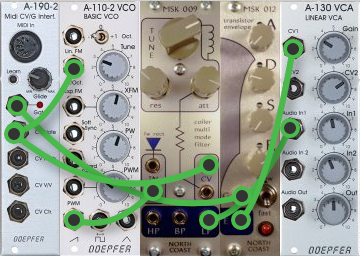
\includegraphics[scale=1.8]{patch1.png}\hspace*{\fill}\par} 

This low-pass gate patch gives an organic sound.  The
tuning knob is turned to its minimum and the envelope output just goes
straight to frequency CV.  Between notes, the envelope voltage is low enough
to tune the filter cutoff below the audio, cutting off the signal.

\nopagebreak\noindent
{\hspace*{\fill}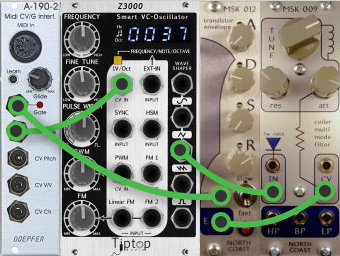
\includegraphics[scale=1.8]{patch3.png}\hspace*{\fill}\par} 

\pagebreak

Deluxe subtractive voice with stereo effect.  There are two oscillators (in
this case, Intellijel Dixie II modules), which could be tuned to near-unison
or a musical interval.  One is patched to the regular audio input of the
Coiler, and one to the rectifier.  There are separate ADSR envelopes for
filter cutoff and amplitude envelope.  The amplitude envelope is applied
independently to the BP and LP outputs of the Coiler, using both channels of
the VCA, and then those two signals go to an MSK~008 octave switch operating
as a ``mid-side decoder''; that is, it computes the sum and difference.  The
two channel outputs of the octave switch are the left and right channels of
a stereo signal.  This patch puts the low-pass signal more or less in the
centre of the stereo field, with higher frequencies from the band-pass
output and some phase effects resulting from the interaction of the two,
spread out on the sides.

\nopagebreak\noindent
{\hspace*{\fill}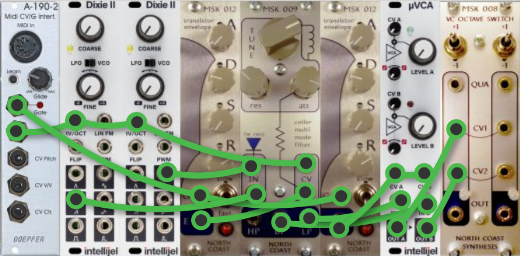
\includegraphics[scale=1.8]{patch2.png}\hspace*{\fill}\par} 

\pagebreak

The Coiler can be used as an oscillator just by turning the resonance knob
all the way up.  It will not track 1V/octave, but for drones with manual
control, and sequencing by ear instead of with a MIDI interface, that makes
little difference.  Sine waves appear on all three outputs, with the purest
one on LP and the most distorted on HP.  Adding a self-patch from the BP
output to the frequency CV, as shown, creates some extra distortion in the
waveform; with some adjustment of the CV attenuation knob, it's possible to
get a reasonable sawtooth wave out of this patch.

\nopagebreak\noindent
{\hspace*{\fill}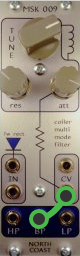
\includegraphics[scale=1.8]{patch4.png}\hspace*{\fill}\par} 

Patch a sine wave LFO into the rectifier input, tune the filter well above
the LFO frequency, and the result is a ``bouncing ball'' CV on the low-pass
output.

\nopagebreak\noindent
{\hspace*{\fill}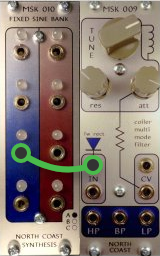
\includegraphics[scale=1.8]{patch5.png}\hspace*{\fill}\par}

\pagebreak

With the tuning set low and audio patched into the rectifier, the Coiler's
low-pass output functions as a simple envelope follower.  In this patch,
it's used as part of a compressor.  The envelope follower goes through an
attenuator/inverter to control an exponential VCA (should be exponential
for good results).  I have shown the Coiler rectifier and VCA audio inputs
patched together, and for standard compression the audio would be applied
that way, to both of them.  For ``sidechain,'' that is, one signal
controlling the compression of another, just feed the main signal into the
VCA and the controlling signal into the Coiler.

\nopagebreak\noindent
{\hspace*{\fill}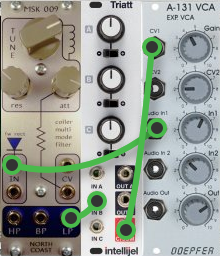
\includegraphics[scale=1.8]{patch6.png}\hspace*{\fill}\par} 
